\chapter{Selection of used technologies}

\thispagestyle{standard}
\pagestyle{standard}

\section{Layer 2 versus Layer 3 device}

Before explaining \acp{VLAN} in detail, it is important to understand the concept of switches. A network switch is used to connect several devices together on a computer network. When speaking about the functionality "switching", a Layer 2 device of the \ac{OSI} model is meant. When performing "switching" the switch uses hardware addresses, in particular the \ac{MAC} address, to forward data from one port to another. \\
Some switches, also known as Multilayer Switches or Layer 3 switches, support "routing functionality", thus referring to a Layer 3 device of the \ac{OSI} model. A Layer 3 device uses \ac{IP} addresses to perform packet forwarding. The most widely known L3 device is the router \cite{wiki:switch}. 

Switches with Layer 2 functionality are used to connect same subnets to each other. In order to enable data communication between different IP subnets, a Layer 3 device with routing functionality is needed! 
Moreover it is important to know, that L2 switches, on the contrary to routers, do not separate broadcast domains. This means, that broadcast messages sent by a client do not traverse a router by default \cite{wiki:switch}.

\section{VLANs}

A \ac{VLAN} is used to allow data communication for a group of devices (e.g. computer, server, firewall and more) as if they were attached to the same wire, although in reality they can be connected to totally different LAN segments (e.g. one device is located in building A and the other device in building B on the other side of the street). \\
Most of the time \acp{VLAN} are associated with \ac{IP} subnets. A \ac{VLAN} defines an own broadcast domain in a Layer 2 network. \acp{VLAN} are typically defined at switches and are based on logical instead of physical connections. \\
Figure \ref{img:example_of_vlans} shows three different \acp{VLAN} that span multiple floors \cite{cisco:vlan}. 

\begin{figure}[ht!]
	\centering
	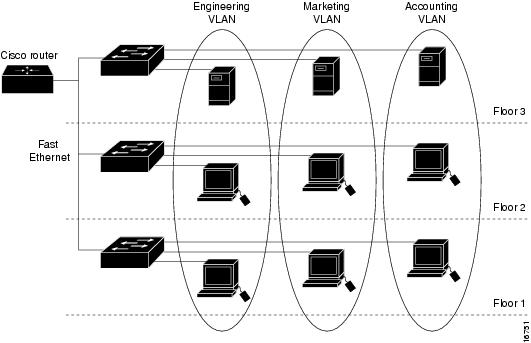
\includegraphics[width=0.9\textwidth]{BilderAllgemein/example_vlans.jpg}
	\caption{Example of VLANs \cite{cisco:vlan}}
	\label{img:example_of_vlans}
\end{figure}

\subsection{Trunks and tagged VLANs}

Trunk links are required to pass several VLANs from one switch to another when using only one logical connection. On a Cisco switch a port can be configured for either access or trunk mode. Access ports belong to only one VLAN and frames exiting such a port are not tagged (marked). Trunk ports on the other way allow the transmission of several VLANs. In order to be able to distinguish the VLAN origin of the frame it is marked with a VLAN tag. This marking procedure is called tagging and uses some tagging mechanism (ISL or 802.1Q, whereby 802.1Q is the most commonly used). \\
A tagged and untagged frame mainly distinguishes between having a VLAN tag or not.

Fig. \ref{img:ethernet_ii_frame} shows the concept of tagging by looking at the most common Ethernet frame type Ethernet-II (IEEE 802.3) including an inserted 802.1Q VLAN tag \cite{ciscopress:vlan}.

\begin{figure}[ht!]
	\centering
	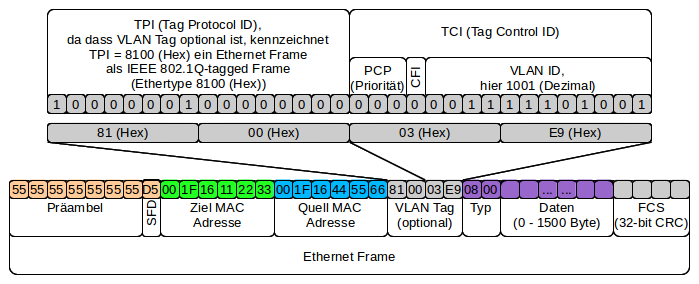
\includegraphics[width=1\textwidth]{BilderAllgemein/vlan_tag.png}
	\caption{Ethernet-II frame with 802.1Q VLAN tag \cite{krenn:tag}}
	\label{img:ethernet_ii_frame}
\end{figure}

\newpage
\textbf{Native VLAN}

The only VLAN that is not tagged on a trunk is called the native VLAN. This means that all packets belonging to the native VLAN do not have a VLAN tag. When configuring a trunk on a Cisco switch and not specifically defining a native VLAN, the native VLAN will be VLAN 1.

\section{Hypervisor}

A hypervisor is a piece of software that allows for one physical device (e.g. computer or server) to share its resources amongst several \acp{VM} running on that physical device. \\
Speaking of terminology, the server that is running the hypervisor is called host machine and the VMs are called guest machines. As displayed in fig. \ref{img:type_1_type_2_hypervisor} the hypervisors are divided into Type-1 (native or bare-metal) hypervisors and Type-2 (hosted) hypervisors \cite{bill:hypervisor}.

\begin{figure}[ht!]
	\centering
	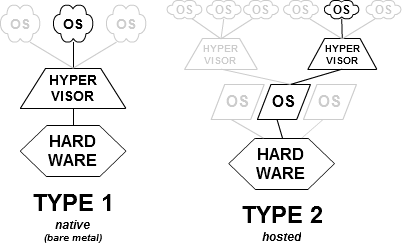
\includegraphics[width=0.8\textwidth]{BilderAllgemein/hypervisor.png}
	\caption{Difference between Type-1 and Type-2 hypervisor \cite{wiki:hypervisor}}
	\label{img:type_1_type_2_hypervisor}
\end{figure}

\textbf{Type-1 Hypervisor}

When installing this type, the hypervisor is directly installed as an operating system. A huge advantage is, that the hypervisor can directly communicate with the underlying physical hardware. These physical hardware resources are then \textit{paravirtualized} and provided to the virtual machines. This type of hypervisor is the preferred method for productive server environments. One hypervisor of this type is VMware ESXi, which has also been used within the IT infrastructure at RITH \cite{bill:hypervisor}.

\textbf{Type-2 Hypervisor}

When speaking of this type, a hypervisor that can be directly installed on an operating system is meant. Two popular freeware products are VMware Player and Oracle VM VirtualBox. These types of hypervisor are not used for productive server environments. They are more used to quickly do some tests and experiments without crashing the own operating system \cite{bill:hypervisor}. 

An example would be that someone would like to test a linux operating system. He/she then installs a Type-2 Hypervisor on his/her operating system (e.g. Windows 10) and creates a VM for Linux. After that he/she is able to do everything within this VM without affecting his/her used operating system Windows 7.

\textbf{Paravirtualization Tools}

These tools (in case of VMware also called VMware Tools) are installed on the VMs to perfectly support the paravirtualized hardware, that is provided by the hypervisor \cite{bill:hypervisor}. 

The following shows an example regarding the Paravirtualization Tools. \\
The hypervisor is accessing the \ac{NIC} of the physical server and paravirtualizing it, in order to provide this specific \ac{NIC} to several VMs. When creating the VM, this paravirtualized \ac{NIC} is then chosen as the network card for the VM. To get optimal performance, the Paravirtualization Tools provide a specific driver for this paravirtualized \ac{NIC}, that can be installed on the OS of the guest machine.

\chapter{IT Infrastructure}

\thispagestyle{standard}
\pagestyle{standard}

\section{Final Hardware}

Regarding the hardware constellation of the main server and the backup server it was important to have a \ac{RAID} controller available in order to obtain reliability. 

\textbf{Storage space design:}

The \acp{HDD} on the main server have been configured to operate in a \ac{RAID} 5. When speaking of \ac{RAID} 5, there always is one \ac{HDD} used for parity purposes, whereby the usable capacity is then reduced by the size of one \ac{HDD}. Furthermore, when configuring a \ac{RAID} 5, every \ac{HDD} has to be the same size. The main server has four 1.2 TB \acp{HDD}. This results in a net capacity (usable capacity) of 3.6 TB. 

The \ac{NAS} has two 6 TB \acp{HDD} and is configured in a \ac{RAID} 1. This type of \ac{RAID} performs a mirroring of hard disks, what means that one \ac{HDD} can be damaged and the data is still available. Due to the RAID 1 the net capacity of the \ac{NAS} results in 6 TB. \\
The backup server is also configured in a \ac{RAID} 5. Based on the five \acp{HDD} with a size of 300 GB each the net capacity is 1.2 TB. \\
Table \ref{tbl:net_capacity_of_components} summarizes the calculations explained above.
\vspace{10pt}

\begin{table}[ht!]
\centering
\begin{tabular}{C{3cm}|C{2cm}|C{5cm}}
\textbf{Component} & \textbf{RAID} & \textbf{Net capacity} \\
\hline
Main Server & 5 & 3.2 TB \\
\hline
Backup Server & 5 & 1.2 TB \\
\hline
NAS & 1 & 6 TB \\
\end{tabular} 
\caption{Net capacity of components}
\label{tbl:net_capacity_of_components}
\end{table}

The limiting component regarding the storage space was the local storage of the backup server. Due to this reason the decision was made to store the backup files on the \ac{NAS}. The backup server only hosts the operating system on the local storage and the actual backup files are accessed from the NAS via the \ac{iSCSI} protocol.

Table \ref{tbl:auflistung_finaler_hardware} shows the hardware components that have been installed at \ac{RITH}.

\begin{table}[ht!]
\centering
\begin{tabular}{C{3cm}|C{3cm}|C{5cm}|C{2cm}}
\textbf{Component} & \textbf{Hardware} & \textbf{Specifications} & \textbf{Support} \\
\hline
Main Server & Fujitsu PY TX1320M2/SFF & - Intel Xeon E3-1230v5 \newline - 3x 12GB DDR4-2133 \newline - 4x SAS 12G 1.2TB \newline - RAID 5/6 Controller \newline - 2x 1GbE RJ45 interface & 5 Year On-Site Service \\
\hline
Backup Server & IBM x3650 M3 & - 2x Intel Xeon E5620 @ 2.40GHz \newline - 3x 4GB \newline - 5x SAS 6G 300GB \newline - RAID 5 Controller \newline - 2x 1GbE RJ45 Interface \newline - Redundant power supply & \\
\hline
KVM Switch & Avocent AUTOVIEW 3016 & \\
\hline
Provider Modem & RAD ASMi-52 & \\
\hline
NAS & 1x Synology DS716+ & & \\
\hline
NAS HDDs & 2x Seagate ST6000VN0021 6TB & & \\
\hline
Switch & 4x Cisco SG300-28 & & \\
\hline
Switch & 2x Cisco SG300-52 & & \\
\hline
Access Points & 6x Cisco WAP200 802.11g PoE &  \\
\hline
Access Points & 5x Ubiquiti AC AP Pro & Including \ac{PoE} Injector & \\
\hline
CCTV & 4x Linksys PVC2300 & \\
\hline
CCTV PC & Computer & \\
\hline
Printer & Several & \\
\hline
Computer, Laptops & Several & \\
\end{tabular} 
\caption{Final Hardware}
\label{tbl:auflistung_finaler_hardware}
\end{table}

\section{IT Infrastructure Plan}

\begin{figure}[H]
	\centering
	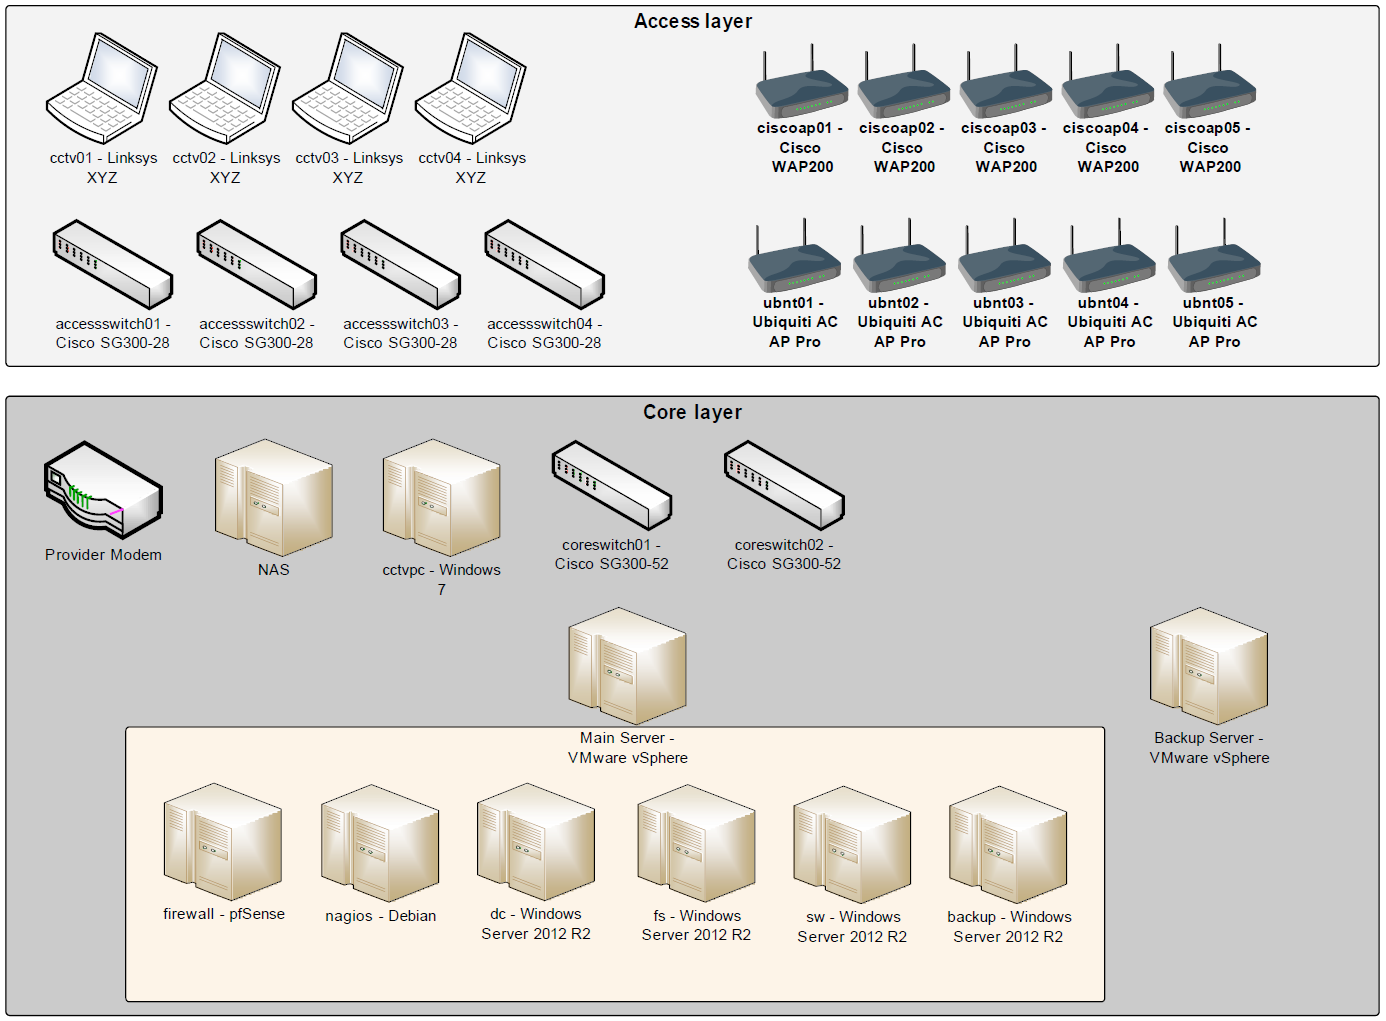
\includegraphics[width=1.0\textwidth]{BilderAllgemein/it_infrastruktur_plan_2.png}
	\caption{IT-Infrastrukturplan}
	\label{img:it_infrastruktur_plan}
\end{figure}

Fig. \ref{img:it_infrastruktur_plan} shows the software and hardware components that were used within the IT infrastructure. It is divided into an access and a core layer. This abstract representation of the IT infrastructure is used to give an overview. Details like \ac{IP} subnets, \ac{IP} addresses, \acp{VLAN}, switch ports or cabling will be shown later.

\subsection{IT Infrastructure Plan in detail}

Core switch 1, as displayed in the plan, establishes the connection between the modem of the \ac{ISP}, the main server, the backup server, the NAS, the CCTV PC, core switch 2 and the remaining access switches. The different IP subnets are separated on the switches by use of VLANs. 

The \ac{OS} of the main server as well as the backup server is VMware vSphere, also called ESXi. Due to this virtualization software, also referred to as hypervisor, several \acp{VM} can be managed on one single physical server. The main server hosts several VMs which are shortly described in the following paragraphs.

On the VM "firewall.ad.rith.edu.bt" the open source operating system pfSense had been installed. This firewall is used to separate and control the traffic between the \ac{WAN} and \ac{LAN} network. Moreover it is used to enable communication between the existing VLANs, which is known as VLAN routing. Monitoring of the WAN bandwidth and WAN quality is also part of the firewall. Therefore the built in graphs called "RRD Graphs", available under Status --> RRD Graphs can be used.

The VM "dc.ad.rith.edu.bt" hosts a Windows Server 2012 R2. This server is used as a domain controller for the local \ac{AD}. The local domain is called "ad.rith.edu.bt". Additionally the server functions as main \ac{DNS} and \ac{DHCP} server for the local network. \acp{GPO} for the \ac{AD} are also created and managed on the domain controller.

Another Windows Server 2012 R2 is installed on the VM "fs.ad.rith.edu.bt". This server's main purpose is to host a file server. Therefore an additional partition "Data (E:)" has been created to save the shared folders. 

The VM "sw.ad.rith.edu.bt" features a Windows Server 2012 R2 too, which is used to host several different software solutions. Currently installed are the UniFi Controller (WiFi controller) for the Ubiquiti access points and the software called Google Active Directory Sync (GADS), which is used to synchronize the user accounts between the Active Directory and Google Apps (Google for Education). \\
Moreover the windows role IIS has been activated, which provides a web server (like Apache). This web server is used to make the software DokuWiki available over the web on the local network.

On the VM "backup.ad.rith.edu.bt" a Windows Server 2012 R2 is installed as operating system. This VM is used to manage the backup between the main server and the backup server. The software that is used for backup is called Veeam Backup\&Replication v9. The backup is done every day at 2am. Details are mentioned in a later section.

The last VM is the "monitoring.ad.rith.edu.bt" on which the operating system Debian 8 has been installed. This VM is used to monitor all the servers and components within the IT infrastructure (e.g. switches, servers, CCTVs and more). The used software is called Check\_MK which relies on Nagios as core service. It is available in a package that comes with several other monitoring solutions. This open source package is called Open Monitoring Distribution (OMD) and can be downloaded from the internet. 

\section{Network Infrastructure}

\subsection{IP Subnets, VLANs and Trunks}

Within the network infrastructure IP subnets have been created. A VLAN ID and one or no DHCP scopes have been assigned to the IP subnets. The size of the subnet has been designed dependent on the number of hosts. The IP network used as basis for subnetting was the private class B net 172.16.0.0/12.

In order to enable communication between the VLANs, a layer 3 device with routing functionality had to be chosen. Within this IT infrastructure the firewall pfSense is accomplishing that task. 

Table \ref{tbl:uebersicht_der_vlans} shows the individual VLANs with additional information.

\begin{table}[ht]
\centering
\begin{tabular}{C{1.3cm}|C{2.8cm}|C{3.5cm}|C{2cm}|C{2.8cm}}
\textbf{\ac{VLAN}} & \textbf{Name} & \textbf{IP Subnet} & \textbf{\# Hosts} & \textbf{DHCP Pool}  \\
\hline
5 & WAN & nein & nein & nein \\
\hline
10 & Management & 172.16.10.0/24 & 254 & 172.16.10.200 - 172.16.10.230 \\
\hline
20 & Internal & 172.16.20.0/22 & 1022 & 172.16.20.50 - 172.16.23.254 \\
\hline
30 & Unifi & 172.16.30.0/27 & 254 & 172.16.30.10 - 172.16.30.30 \\
\end{tabular} 
\caption{Übersicht der VLANs}
\label{tbl:uebersicht_der_vlans}
\end{table}

As seen in table \ref{tbl:uebersicht_der_vlans} VLAN 5 is not assigned to an IP subnet. This is, because the only purpose of VLAN 5 is to separate the WAN traffic from the entire other network. The modem of the \ac{ISP} is connected directly to one port of core switch 1, which has been configured as an access port in VLAN 5. Moreover, only the trunk between core switch 1 and main server, as well as core switch 1 and backup server allows traffic for VLAN 5. On the respective server the trunk then gets split up and only the WAN interface of the VM "firewall.ad.rith.edu.bt", which actually is the WAN interface of the firewall pfSense, gets access to VLAN 5. 

By use of this topology it is ensured, that the modem of the \ac{ISP} is solely connected to the WAN interface of the firewall. The WAN interface of the firewall then receives a DHCP lease of the DHCP server from the \ac{ISP}.

\subsubsection{Trunks}

The connection between the individual switches, between core switch 1 and main server, as well as between core switch 1 and backup server are configured as a trunk, to transmit more than one VLAN over one logical connection. Moreover the connection between the switches and access points are configured as a trunk too. Table \ref{tbl:uebersicht_der_trunks} shows an overview of all established trunks within this network infrastructure.

\begin{table}[H]
\centering
\begin{tabular}{C{3cm}|C{3cm}|C{3cm}|C{3cm}}
\textbf{HW 1} & \textbf{HW 2} & \textbf{Native VLAN} & \textbf{Tagged VLAN} \\
\hline
Coreswitch 1 & Coreswitch 2 & 1 & 10,20,30 \\
\hline
Coreswitch 1 & Main Server & 1 & 5,10,20,30 \\
\hline
Coreswitch 1 & Backup Server & 1 & 5,10,20,30 \\
\hline
Coreswitch 1 & Accessswitch 1 & 1 & 10,20,30 \\
\hline
Coreswitch 1 & Accessswitch 2 & 1 & 10,20,30 \\
\hline
Coreswitch 1 & Accessswitch 3 & 1 & 10,20,30 \\
\hline
Accessswitch 4 & Accessswitch 1 & 1 & 10,20,30 \\
\hline
Switch & Cisco WAP200 & 1 & 10,20 \\
\hline
Switch & Ubiquiti AC AP Pro & 30 & 10,20 \\
\end{tabular} 
\caption{Overview Trunks}
\label{tbl:uebersicht_der_trunks}
\end{table}

The connection between switches and access points has been configured as a trunk in order to transmit VLAN 10 and VLAN 20 tagged. Both the Ubiquiti access points and the Cisco access points distribute two wireless networks. The wireless network with the SSID (name) RITH provides access to VLAN 20, which is used as the default wireless network for students, teacher and members of staff to access the internet and internal network resources. The wireless network with the SSID "RITH Management" connects to VLAN 10 and is only used for management purposes by IT administrators.

The Cisco WAP200 access points receive its management IP address from the DHCP server in VLAN 10. The Ubiquiti access points cannot obtain a management IP address from a network and distribute that network over WiFi at the same time. Therefore a separate IP subnet with the VLAN ID 30 has been created. This VLAN was set as native VLAN on the trunk, because the access point is not capable of maintaining a DHCP lease for its management IP address from a tagged VLAN. 

\subsection{Redundancy and Link Aggregation}

One goal when designing the IT infrastructure was to provide as much redundancy as possible, in order to improve availability as well as reliability. Fig. \ref{img:redundanz_in_der_netzwerkinfrastruktur} shows the cabling of the individual network components.

\begin{figure}[ht!]
	\centering
	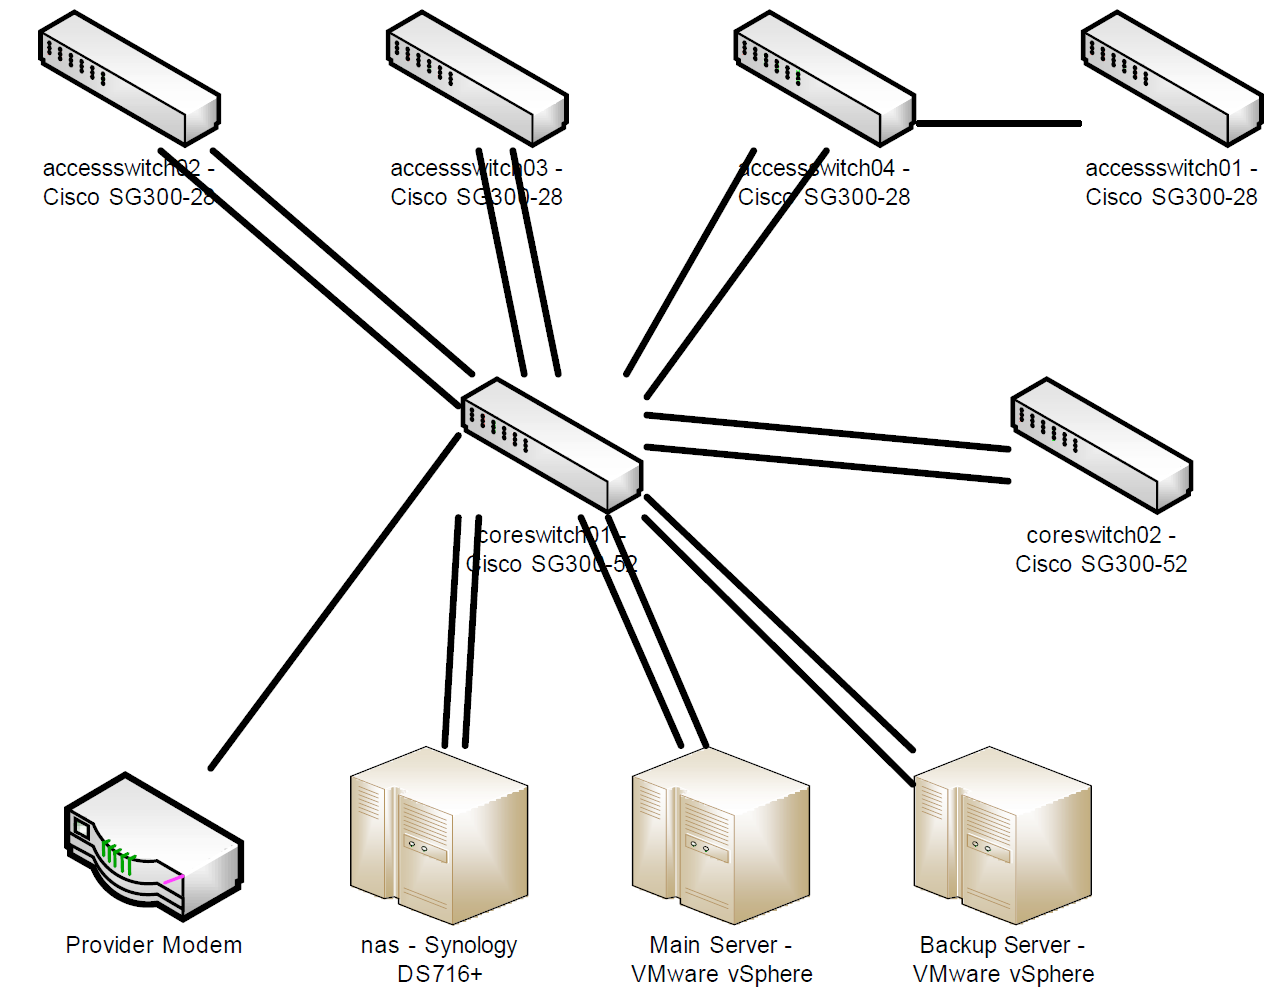
\includegraphics[width=0.8\textwidth]{BilderAllgemein/redundanz.png}
	\caption{Redundancy within the IT infrastructure}
	\label{img:redundanz_in_der_netzwerkinfrastruktur}
\end{figure}

To achieve redundancy between the switches, two instead of just one cable were laid. Each port on a switch, that was belonging to the same logical connection, was assigned to a \ac{LAG}. On the Cisco SG300 switches those \acp{LAG} are called port-channels. The configuration for those port-channels had to be the same on both switches. Furthermore the \ac{LACP} has been deactivated on both sides. The following listing shows the commands for the Cisco SG300 switch to achieve this configuration. Lines starting with an exclamation mark are comments.

\begin{lstlisting}
! assign the corresponding interfaces to a port-channel
coreswitch01(config)#interface gigabitethernet 49
coreswitch01(config-if)#channel-group 2 mode on
coreswitch01(config-if)#exit
coreswitch01(config)#interface gigabitethernet 50
coreswitch01(config-if)#channel-group 2 mode on
coreswitch01(config-if)#exit

! set the vlan configuration on the port-channel and not on 
! the interfaces
coreswitch01(config)#interface port-channel 2
coreswitch01(config-if)#description "to coreswitch02"
coreswitch01(config-if)#switchport mode trunk
coreswitch01(config-if)#switchport trunk allowed vlan add 10,
                        20,30
\end{lstlisting} 

Speaking of the redundant communication between core switch 1 and main server, as well as core switch 1 and backup server, all configuration had been made on the ESXi. On the core switch 1 itself no special configuration regarding \ac{LA} had to be made. \\
ESXi ensures redundancy, that means that all physical links except of one can fail. Moreover it makes load balancing between the physical links, so that the load is distributed equally upon all physical connections.

For the connection between core switch 1 and \ac{NAS} a \ac{LAG} has been created and \ac{LACP} enabled in passive mode. This is a requirement from the \ac{NAS} to get a working \ac{LA}. In addition, the port-channel connected to the NAS has been configured as an access port in VLAN 10. \\
The following listing shows the used commands to achieve that configuration on a Cisco SG300 switch.

\begin{lstlisting}
! assign the corresponding interfaces to a port-channel
coreswitch01(config)#interface gigabitethernet 5
coreswitch01(config-if)#channel-group 1 mode auto
coreswitch01(config-if)#exit
coreswitch01(config)#interface gigabitethernet 6
coreswitch01(config-if)#channel-group 1 mode auto
coreswitch01(config-if)#exit

! set the vlan configuration on the port-channel and not on 
! the interfaces
coreswitch01(config)#interface port-channel 1
coreswitch01(config-if)#description "to NAS"
coreswitch01(config-if)#switchport mode access
coreswitch01(config-if)#switchport access vlan 10
\end{lstlisting} 

\subsection{vSphere Network Configuration}

\begin{figure}[H]
	\centering
	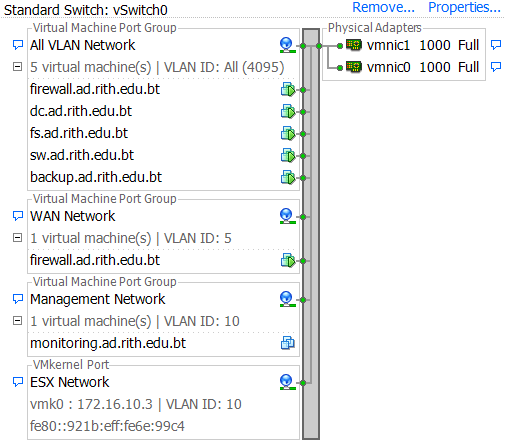
\includegraphics[width=0.8\textwidth]{BilderAllgemein/netzwerkkonfiguration_esxi.png}
	\caption{Network configuration ESXi main server}
	\label{img:netzwerkkonfiguration_esxi_main_server}
\end{figure}

Fig. \ref{img:netzwerkkonfiguration_esxi_main_server} shows the virtual network configuration of 1vSphere on the main server. As displayed, two physical network adapters are assigned to vSwitch0 in order to achieve redundancy and load balancing, as described in the previous chapter. Every network adapter works at 1 Gbps full duplex. \\
Due to the trunk, that has been configured on core switch 1, VLAN tagging has to be done on the vSphere too, in order to identify the different VLANs and successfully split the packets. For example core switch 1 is now tagging all packets that correspond to VLAN 10 with a 802.1Q tag containing the label 10. Only by doing this, the opposite side is then able to identify packets that belong to VLAN 10 by looking at the 802.1Q tag in the header of the IP packet. \\
For example the port group "Management Network", that can be seen in the picture, only handles packets with a 802.1Q tag that contain the VLAN ID 10.

In general two different connection types are distinguished. The VMKernel Port and the Virtual Machine Port Group. The former is a TCP/IP stack to manage traffic for the ESXi services vSphere Motion, iSCSI, NFS and host management. The latter is a virtual network interface that mainly offers three different options: define a specific VLAN ID, allow all VLAN IDs or allow no VLAN ID. \\
When a VLAN ID is specified on the virtual network interface only packets belonging to that VLAN are processed. Moreover the 802.1Q tag gets removed from the packet header. \\
When the virtual network interface is configured to allow all VLAN IDs, every packet containing a 802.1Q tag is processed. Therefore the operating system must take care of the separation of the packets concerning the VLANs. \\
If the virtual network interface is configured for no VLAN ID, only untagged packets will get processed by that interface.

The "ESX Network" of type VMkernel Port, as shown in the figure, is used to process the management traffic for the ESXi host. Only this VMkernel Port has an IP address assigned. The ESXi host is accessible via this configured IP address. \\
On the backup server this network was additionally used to access the iSCSI Target that is located on the NAS.

As seen in the figure the VMs "dc", "fs", "sw" and "backup" are assigned to the "All VLAN Network". That means that the VLAN separation has to be done within the operating system. In order to be able to use that, the network adapter for the VM has to be of the VMXNET3, as seen in figure \ref{img:network_adapter_vmxnet3}. 

\begin{figure}[h!]
	\centering
	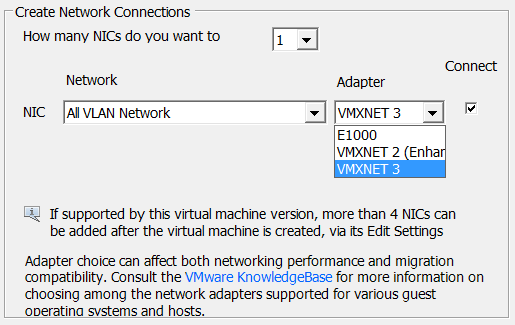
\includegraphics[width=0.6\textwidth]{BilderAllgemein/vmxnet3.png}
	\caption{Network adapter VMXNET3}
	\label{img:network_adapter_vmxnet3}
\end{figure}

After using VMXNET3 as network adapter type and allowing "All VLANs" on the network, the VLAN can be configured within the properties of the specific \ac{NIC} on the operating system. Fig. \ref{img:configuring_vlan_id_on_nic} shows the procedure in case of a Windows Server 2012 R2.

\begin{figure}[h!]
	\centering
	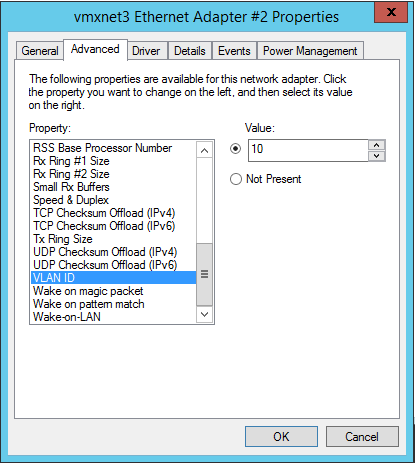
\includegraphics[width=0.6\textwidth]{BilderAllgemein/vmxnet3_properties.png}
	\caption{Configuring VLAN ID on NIC}
	\label{img:configuring_vlan_id_on_nic}
\end{figure}

The WAN interface of the VM "firewall" was connected to a network with the VLAN ID 5 and the LAN interface also the network with all VLANs allowed. 

The debian based VM "monitoring" was connected to a network for VLAN 10, because only one VLAN was needed and thus no VLAN configuration within the operating system had to be made.



